\documentclass[border=10pt,tikz]{standalone}
\usepackage{amsmath}
\usepackage{amssymb}
\usepackage{bm}
\usepackage{tikz}
\usetikzlibrary{arrows.meta,calc,decorations.pathreplacing,patterns,shapes.geometric,positioning,shadings}

\begin{document}
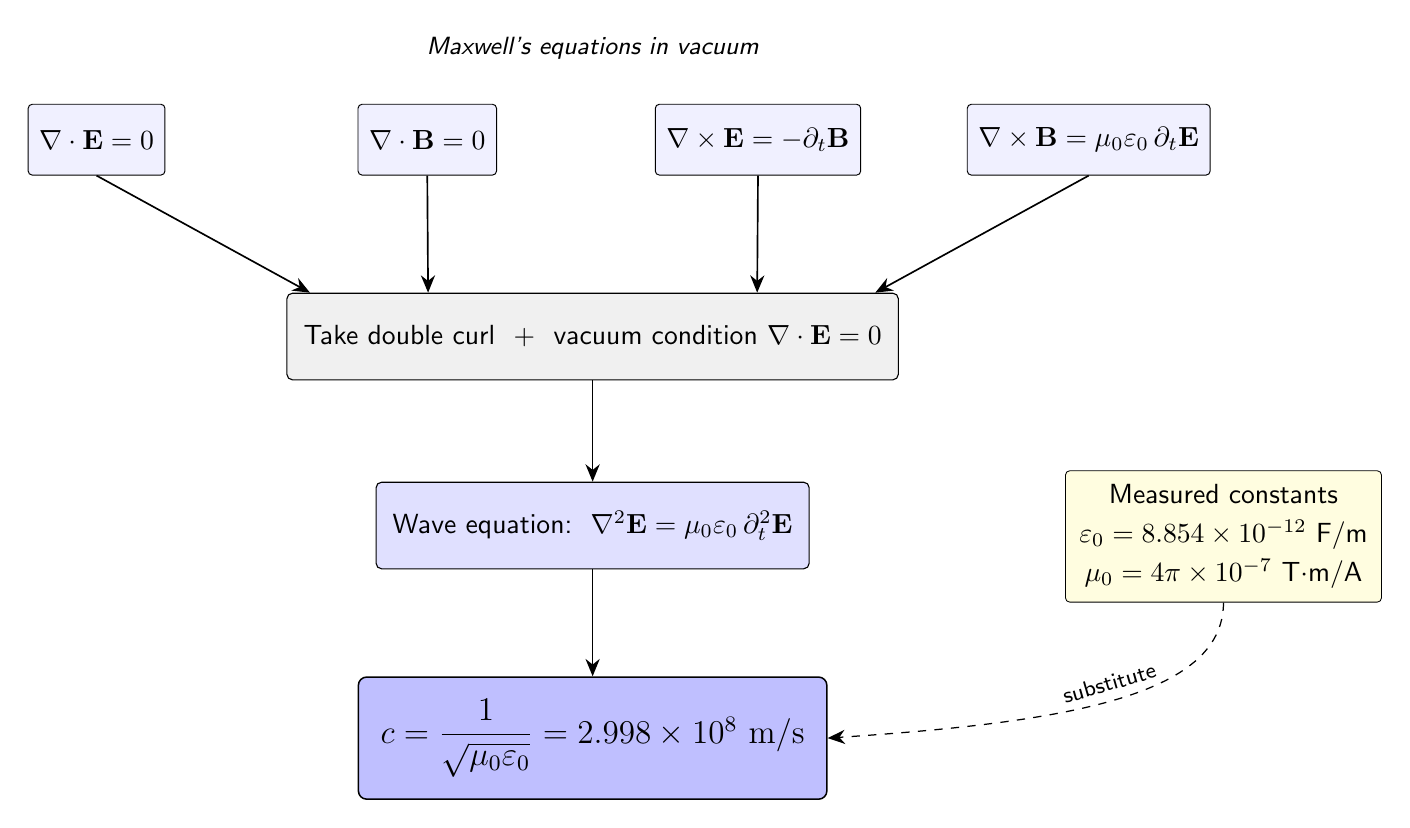
\begin{tikzpicture}[
  font=\sffamily,
  >={Stealth[length=2.2mm,width=1.8mm]},
  eqbox/.style={
    draw=black,
    line width=0.35pt,
    fill=blue!6,
    rounded corners=1.5pt,
    inner sep=4pt,
    minimum height=9mm,
    align=center
  },
  stepbox/.style={
    draw=black,
    line width=0.4pt,
    fill=gray!12,
    rounded corners=2pt,
    inner sep=6pt,
    minimum height=11mm,
    align=center
  },
  wavebox/.style={
    draw=black,
    line width=0.4pt,
    fill=blue!12,
    rounded corners=2pt,
    inner sep=6pt,
    minimum height=11mm,
    align=center
  },
  resultbox/.style={
    draw=black,
    line width=0.55pt,
    fill=blue!25,
    rounded corners=3pt,
    inner sep=8pt,
    minimum height=14mm,
    align=center
  },
  constbox/.style={
    draw=black,
    line width=0.3pt,
    fill=yellow!12,
    rounded corners=1.5pt,
    inner sep=5pt,
    align=center
  },
  flow/.style={->, line width=0.6pt, black},
  dashflow/.style={->, line width=0.45pt, black, dashed}
]

% Top row: four Maxwell equations
\node[eqbox] (e1) at (-6.3, 4.2) {$\nabla\cdot\mathbf{E}=0$};
\node[eqbox] (e2) at (-2.1, 4.2) {$\nabla\cdot\mathbf{B}=0$};
\node[eqbox] (e3) at ( 2.1, 4.2) {$\nabla\times\mathbf{E}=-\partial_t\mathbf{B}$};
\node[eqbox] (e4) at ( 6.3, 4.2) {$\nabla\times\mathbf{B}=\mu_0\varepsilon_0\,\partial_t\mathbf{E}$};

% Header label above equations
\node[anchor=south, font=\sffamily\small\itshape] at (0, 5.1) {Maxwell's equations in vacuum};

% Middle step box: take double curl + vacuum condition
\node[stepbox] (step) at (0, 1.7) {Take double curl\ \ $+$\ \ vacuum condition $\nabla\cdot\mathbf{E}=0$};

% Arrows from four equations into step box
\draw[flow] (e1.south) -- ($(step.north west)+(0.3,0)$);
\draw[flow] (e2.south) -- ($(step.north west)+(1.8,0)$);
\draw[flow] (e3.south) -- ($(step.north east)+(-1.8,0)$);
\draw[flow] (e4.south) -- ($(step.north east)+(-0.3,0)$);

% Wave equation box
\node[wavebox] (wave) at (0, -0.7) {Wave equation:\ \ $\nabla^{2}\mathbf{E}=\mu_0\varepsilon_0\,\partial_t^{2}\mathbf{E}$};

% Arrow from step to wave
\draw[flow] (step.south) -- (wave.north);

% Result box
\node[resultbox, font=\sffamily\large] (res) at (0, -3.4)
  {$c=\dfrac{1}{\sqrt{\mu_0\varepsilon_0}}=2.998\times 10^{8}\ \mathrm{m/s}$};

% Arrow from wave to result
\draw[flow] (wave.south) -- (res.north);

% Right-side constants column
\node[constbox, anchor=north west] (c1) at (6.0, 0.0)
  {Measured constants\\[2pt]$\varepsilon_0 = 8.854\times 10^{-12}$\ F/m\\[2pt]$\mu_0 = 4\pi\times 10^{-7}$\ T$\cdot$m/A};

% Dashed arrow from constants into result box, meaning "substitute"
\draw[dashflow] (c1.south) .. controls +(0,-1.2) and +(3.0,0.2) .. (res.east)
  node[midway, above, font=\sffamily\footnotesize, sloped] {substitute};

\end{tikzpicture}
\end{document}
